\subsection{Эмпирическая функция распределения}
\begin{figure}[H]
	\centering
	{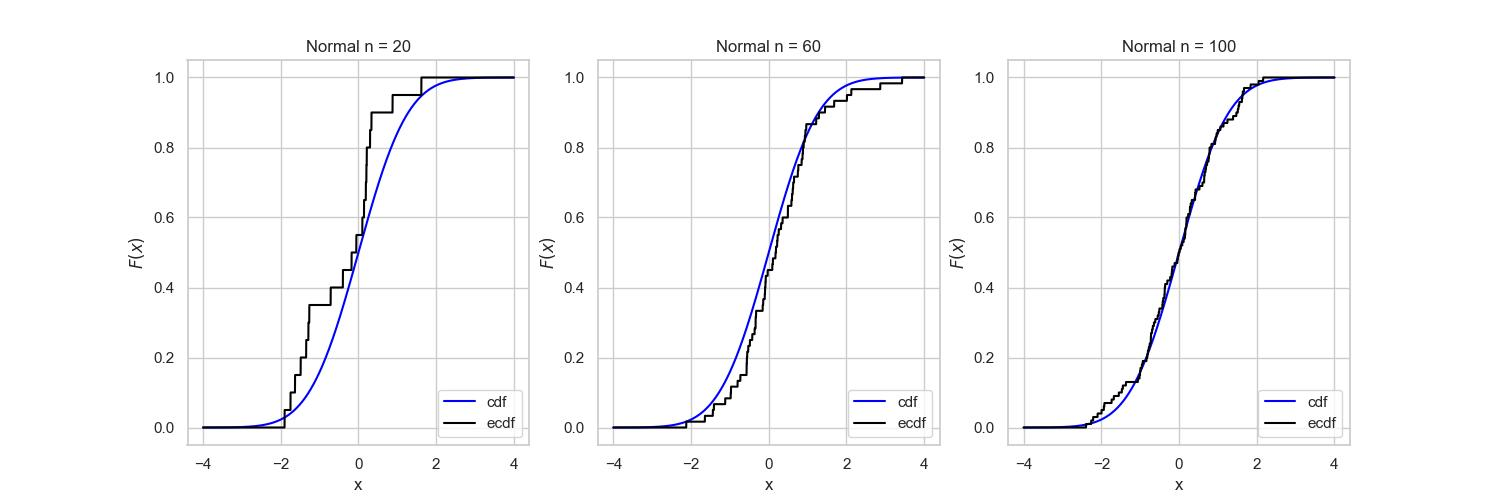
\includegraphics[scale=0.5]{task_4/resource/NormalEmp.jpg}}
		\caption{Нормальное распределение} 
		\label{fig:normal}
\end{figure}

\begin{figure}[H]
	{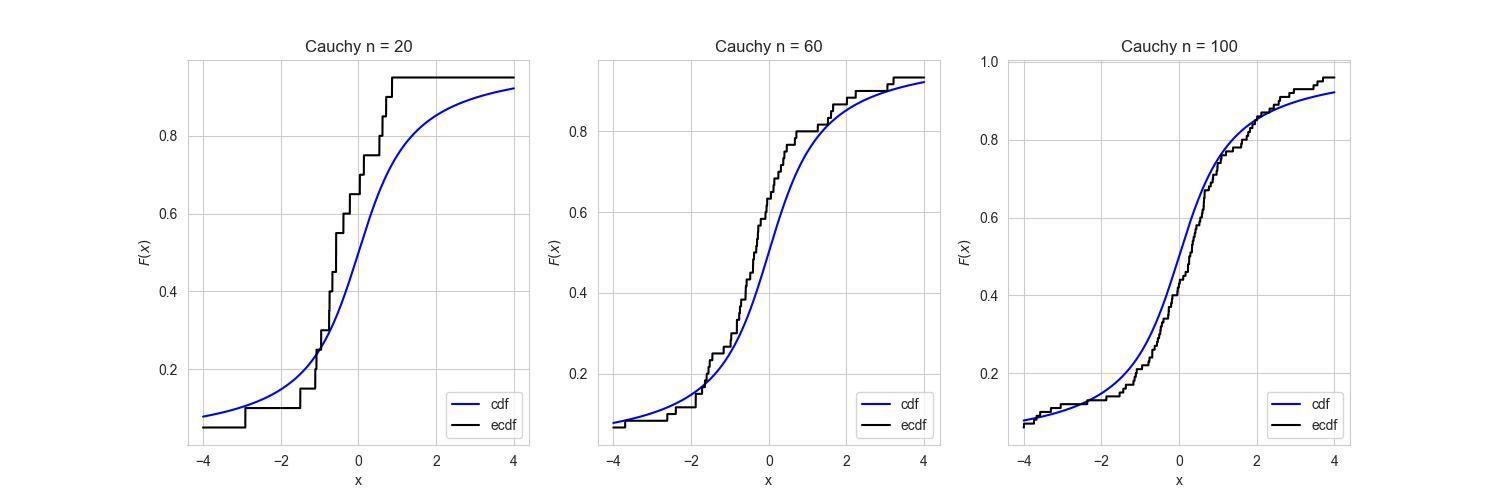
\includegraphics[scale=0.5]{task_4/resource/CauchyEmp.jpg}}
		\caption{Распределение Коши} 
		\label{fig:normal}
	\end{figure}

\begin{figure}[H]
	{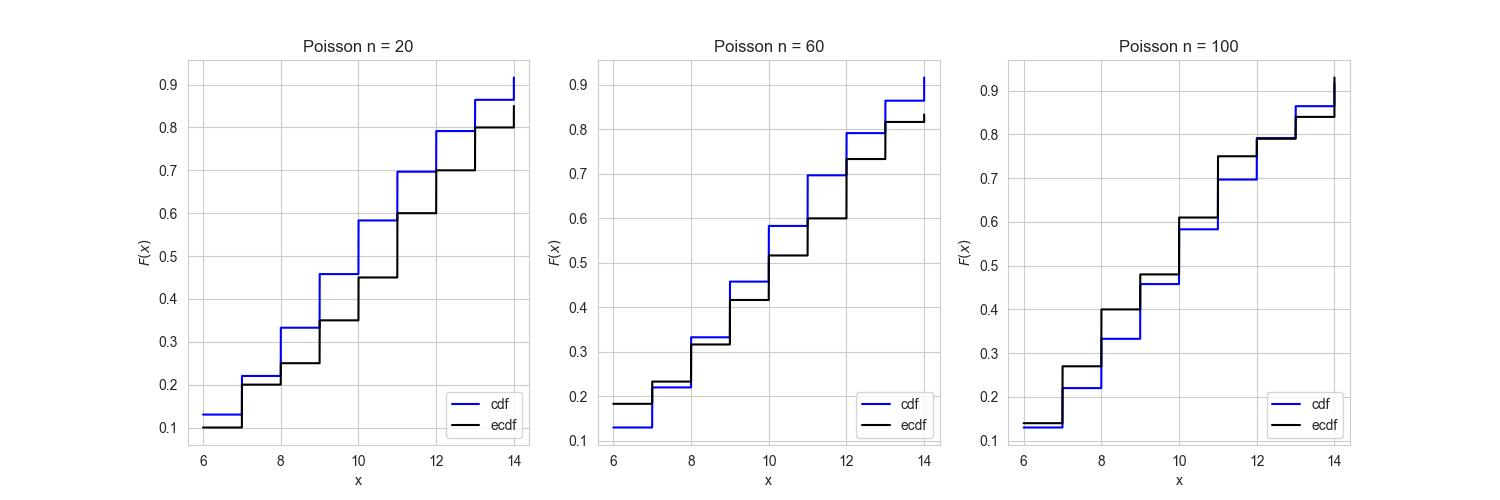
\includegraphics[scale=0.5]{task_4/resource/PoissonEmp.jpg}}
		\caption{Распределение Пуассона} 
		\label{fig:normal}
	\end{figure}
	
\begin{figure}[H]
	{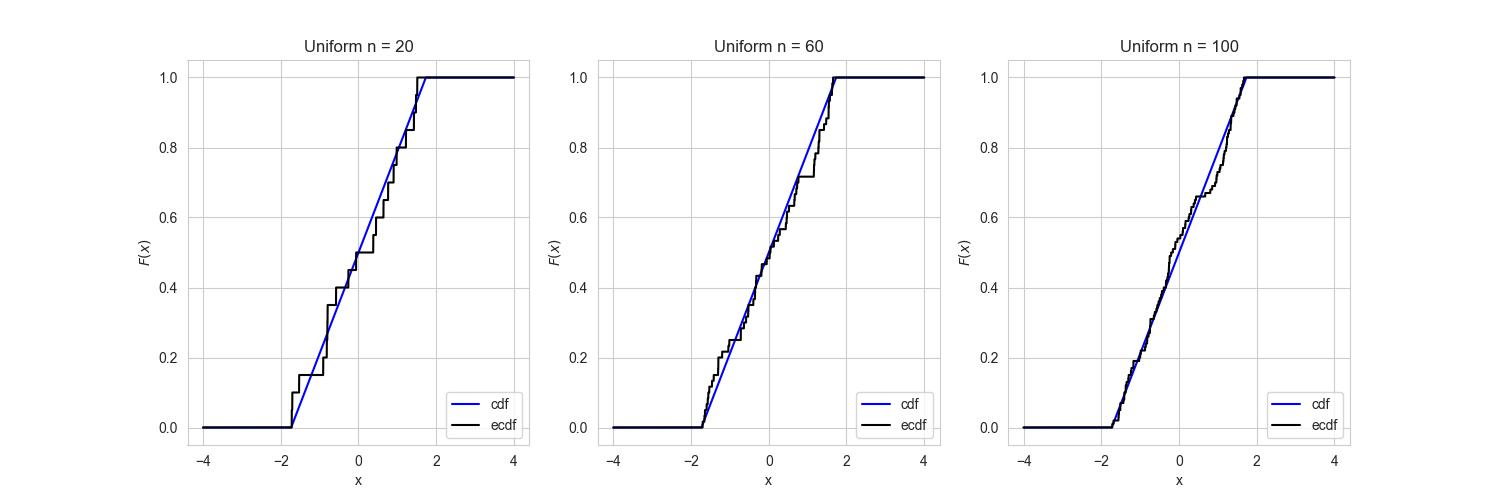
\includegraphics[scale=0.5]{task_4/resource/UniformEmp.jpg}}
		\caption{Равномерное распределение} 
		\label{fig:normal}
	\end{figure}
	
\subsection{Ядерные оценки плотности распределения}
\begin{figure}[H]
	{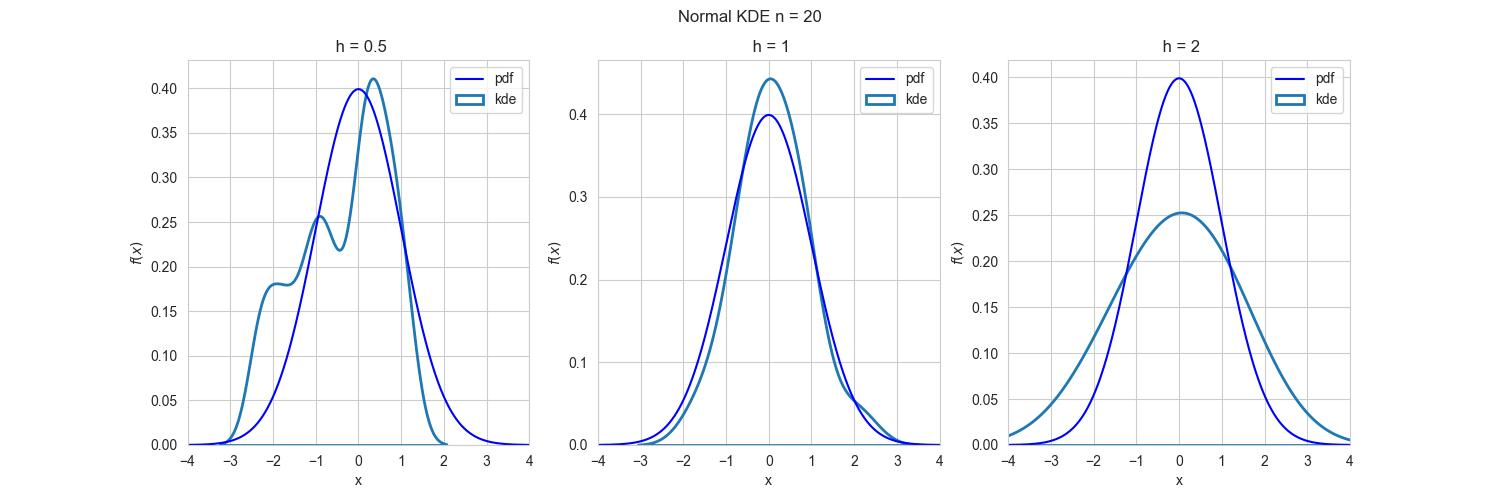
\includegraphics[scale=0.45]{task_4/resource/Normal KDE20.jpg}}
		\caption{Нормальное распределение, $n=20$} 
		\label{fig:normal}
	\end{figure}
	
\begin{figure}[H]
	{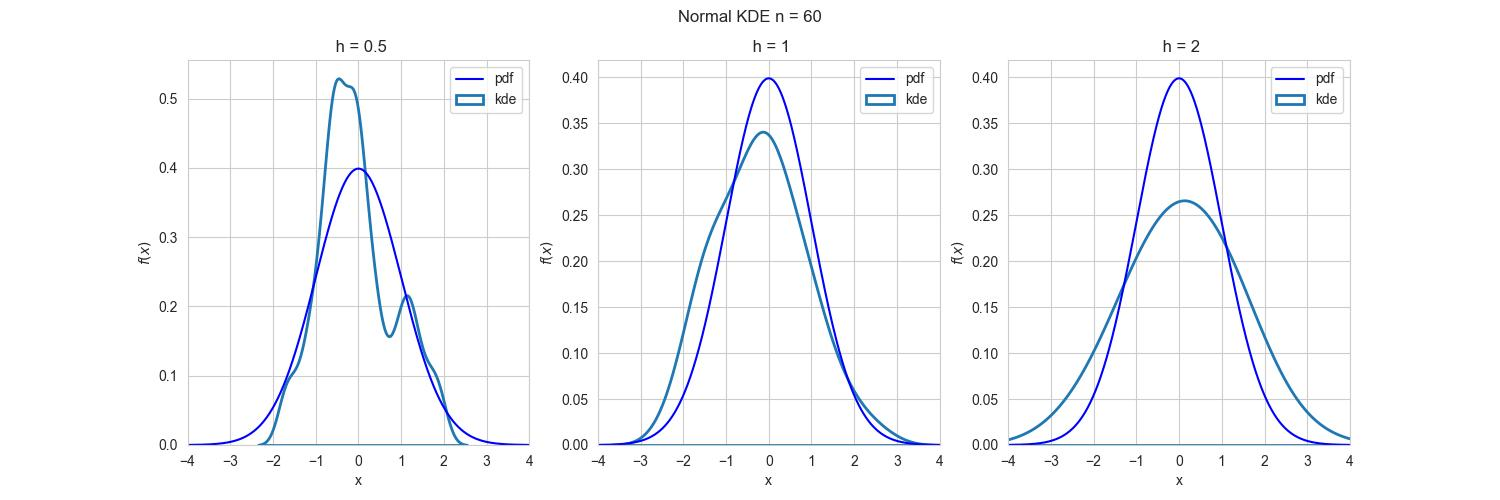
\includegraphics[scale=0.45]{task_4/resource/Normal KDE60.jpg}}
		\caption{Нормальное распределение, $n=60$} 
		\label{fig:normal}
	\end{figure}
		
\begin{figure}[H]
	{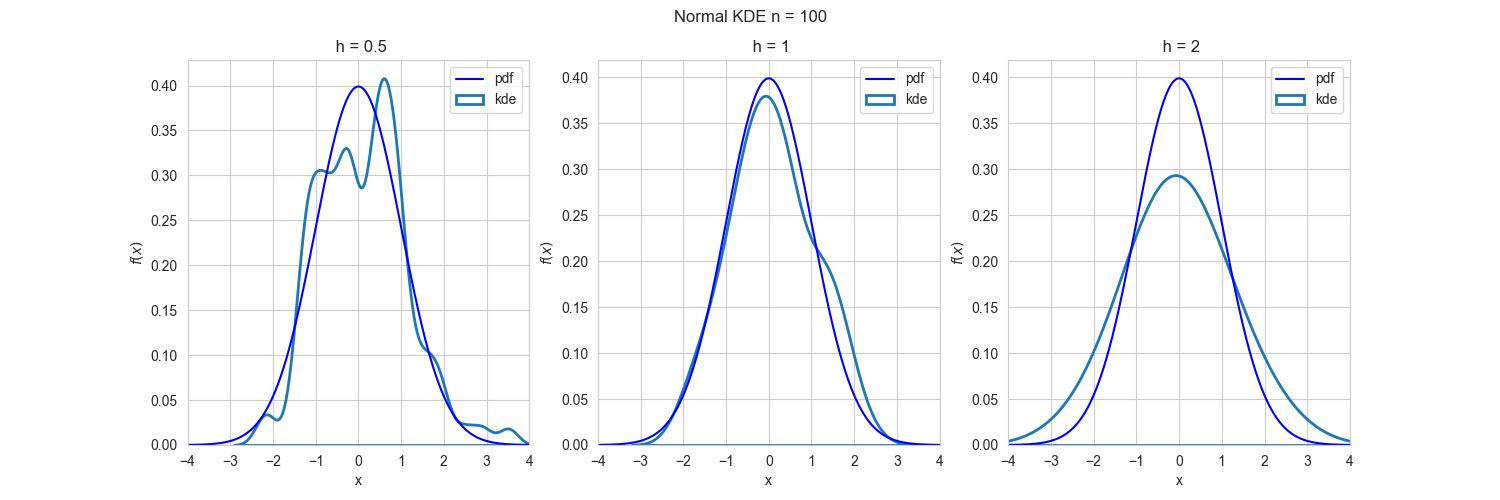
\includegraphics[scale=0.45]{task_4/resource/Normal KDE100.jpg}}
		\caption{Нормальное распределение, $n=100$} 
		\label{fig:normal}
	\end{figure}

\begin{figure}[H]
	{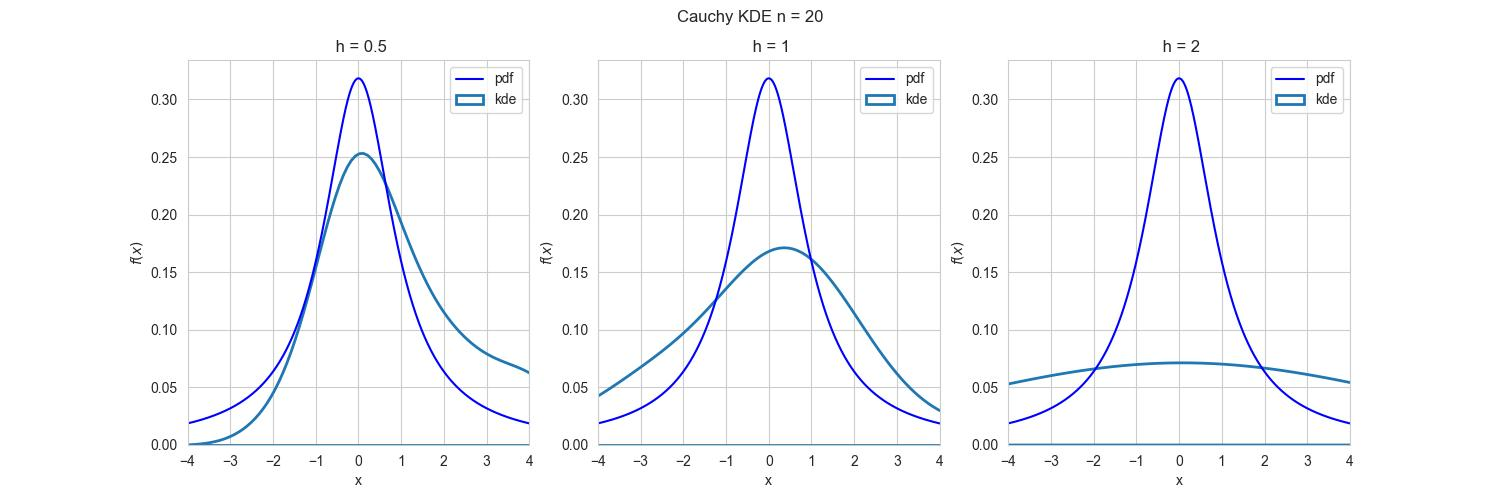
\includegraphics[scale=0.45]{task_4/resource/Cauchy KDE20.jpg}}
		\caption{Распределение Коши, $n=20$} 
		\label{fig:normal}
	\end{figure}
	
\begin{figure}[H]
	{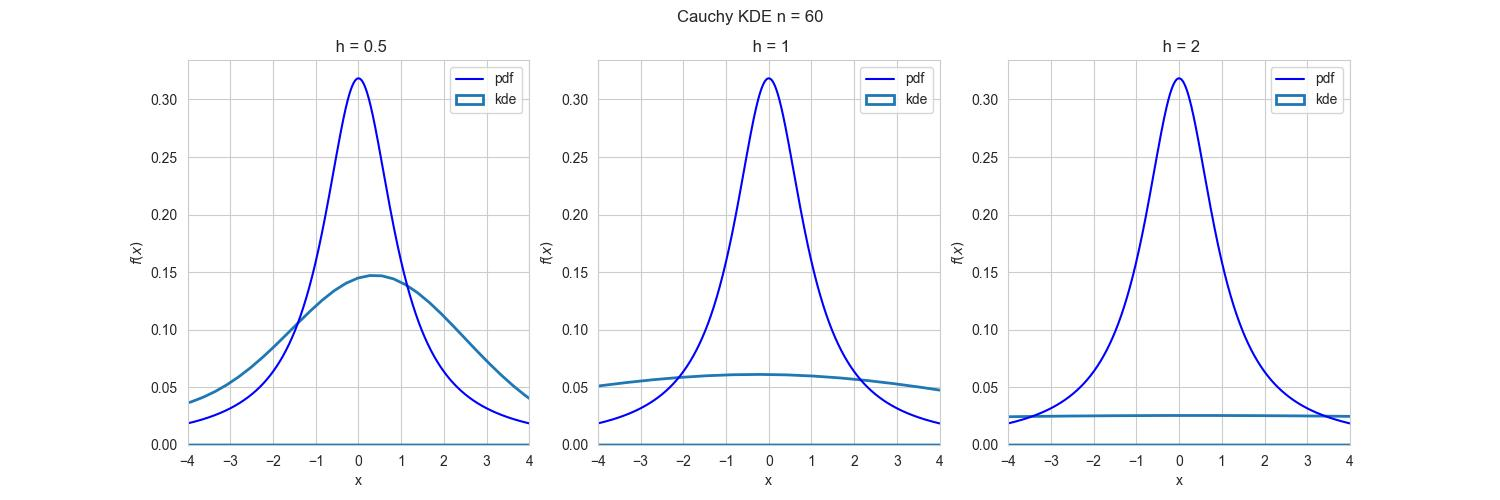
\includegraphics[scale=0.45]{task_4/resource/Cauchy KDE60.jpg}}
		\caption{Распределение Коши, $n=60$} 
		\label{fig:normal}
	\end{figure}
	
\begin{figure}[H]
	{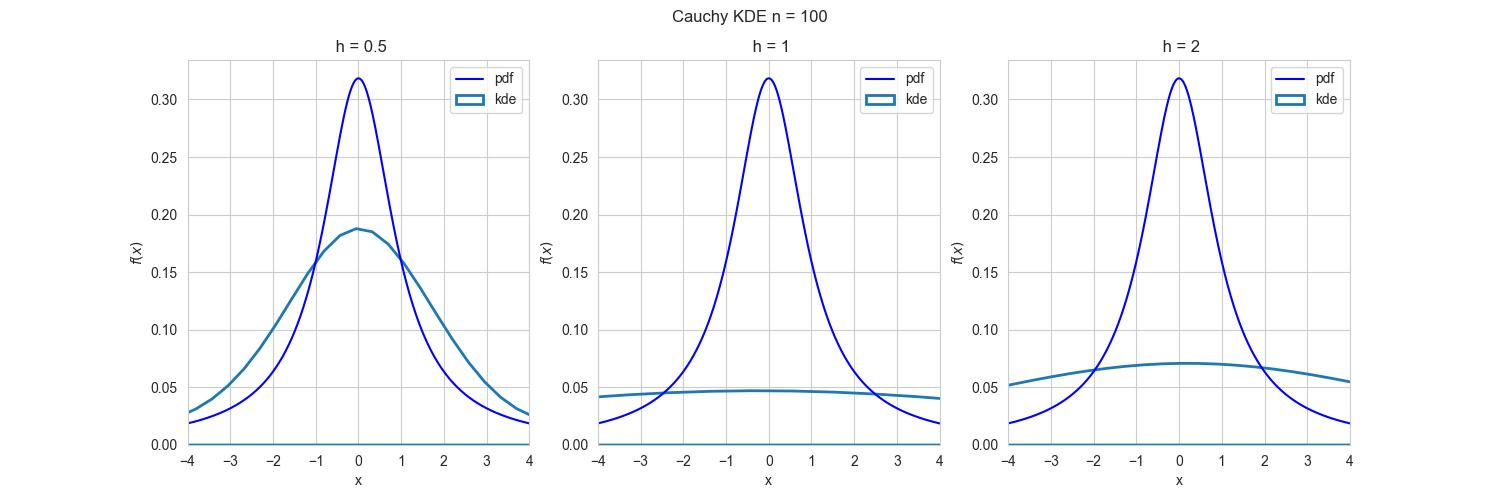
\includegraphics[scale=0.45]{task_4/resource/Cauchy KDE100.jpg}}
		\caption{Распределение Коши, $n=100$} 
		\label{fig:normal}
	\end{figure}

\begin{figure}[H]
	{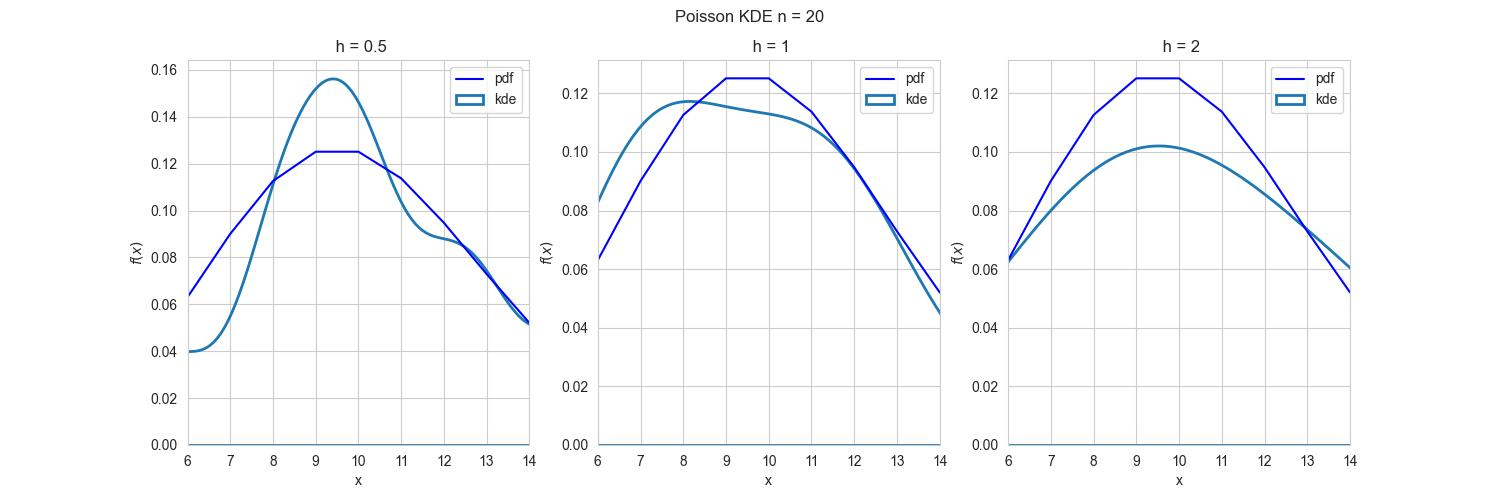
\includegraphics[scale=0.45]{task_4/resource/Poisson KDE20.jpg}}
		\caption{Распределение Пуассона, $n=20$} 
		\label{fig:normal}
	\end{figure}
	
\begin{figure}[H]
	{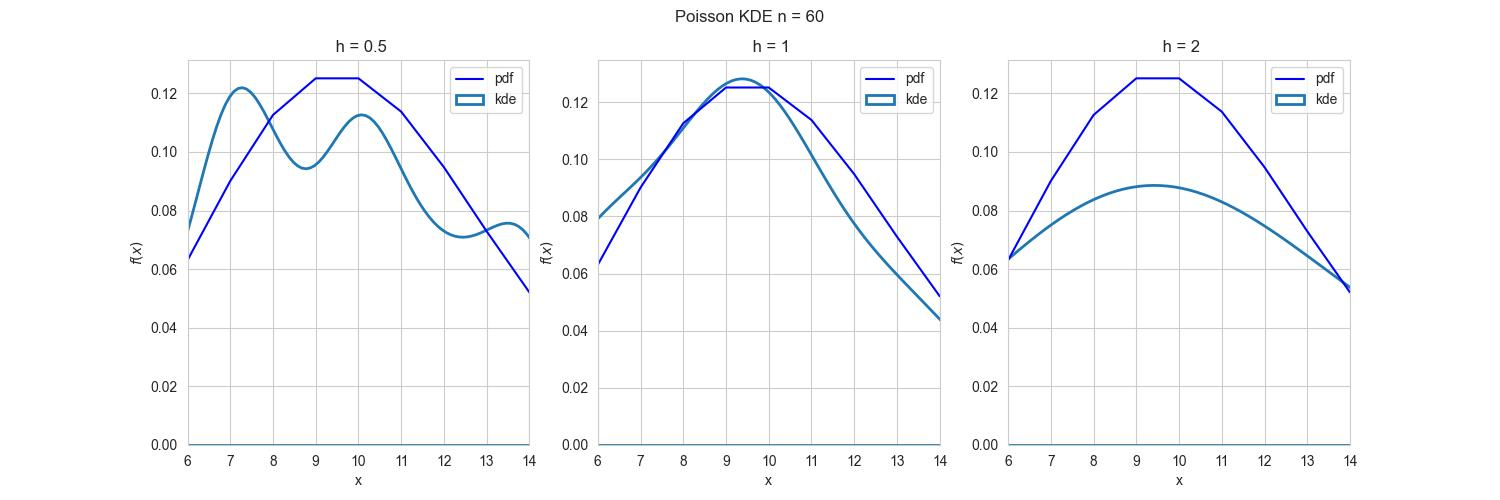
\includegraphics[scale=0.45]{task_4/resource/Poisson KDE60.jpg}}
		\caption{Распределение Пуассона, $n=60$} 
		\label{fig:normal}
	\end{figure}
	
\begin{figure}[H]
	{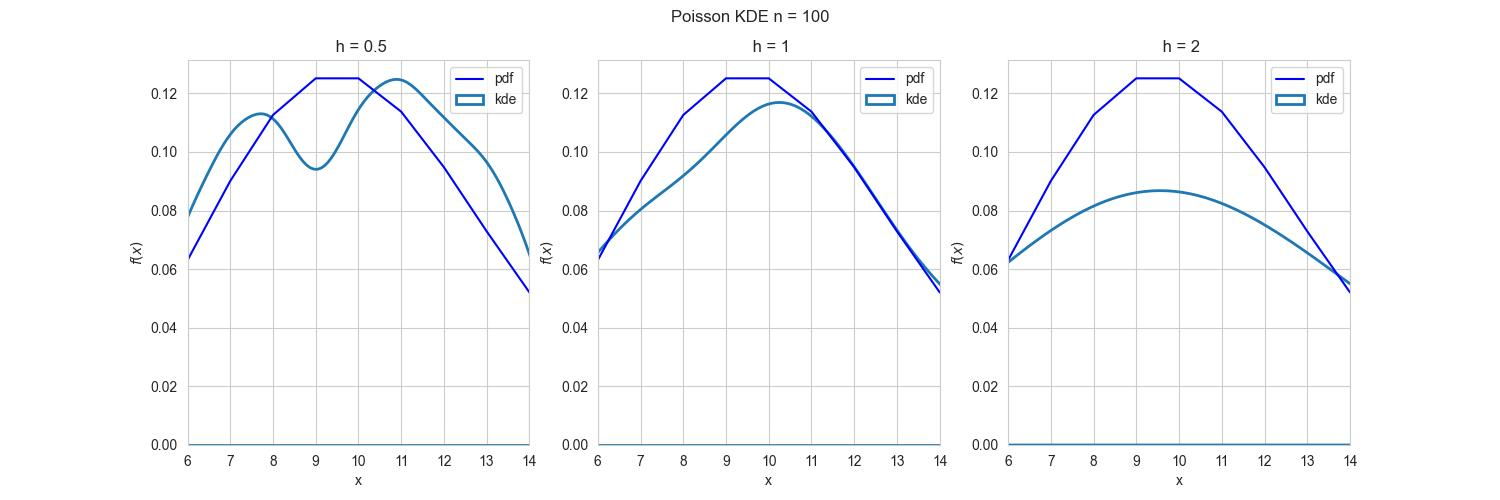
\includegraphics[scale=0.45]{task_4/resource/Poisson KDE100.jpg}}
		\caption{Распределение Пуассона, $n=100$} 
		\label{fig:normal}
	\end{figure}
	
\begin{figure}[H]
	{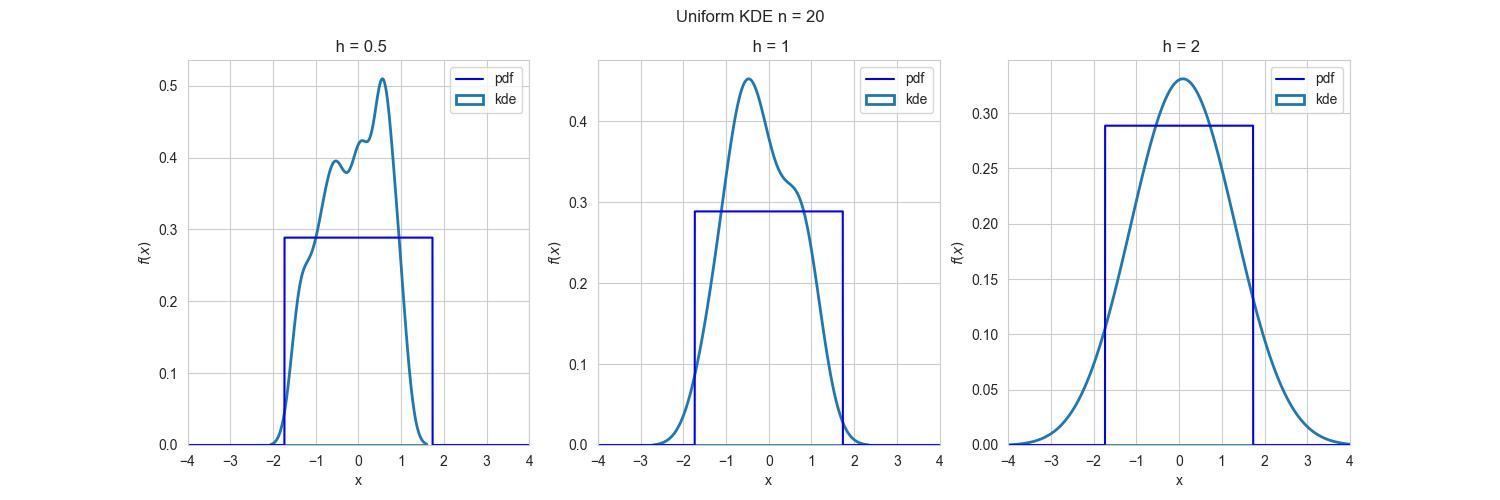
\includegraphics[scale=0.45]{task_4/resource/Uniform KDE20.jpg}}
		\caption{Равномерное распределение, $n=20$} 
		\label{fig:normal}
	\end{figure}
	
\begin{figure}[H]
	{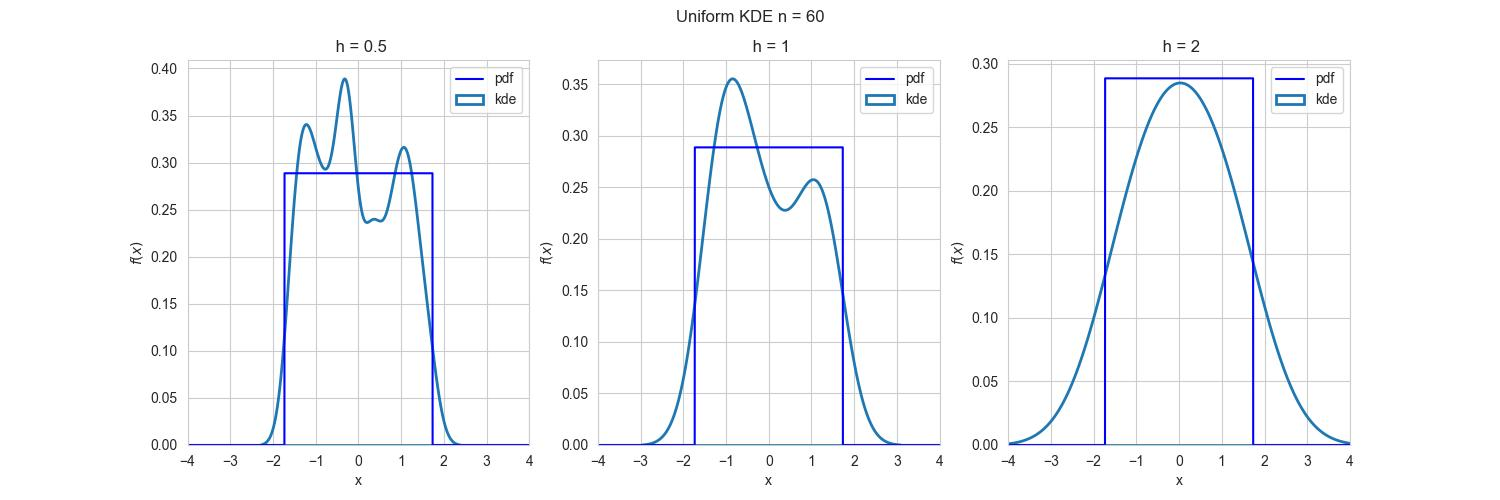
\includegraphics[scale=0.45]{task_4/resource/Uniform KDE60.jpg}}
		\caption{Равномерное распределение, $n=60$} 
		\label{fig:normal}
	\end{figure}

\begin{figure}[H]
	{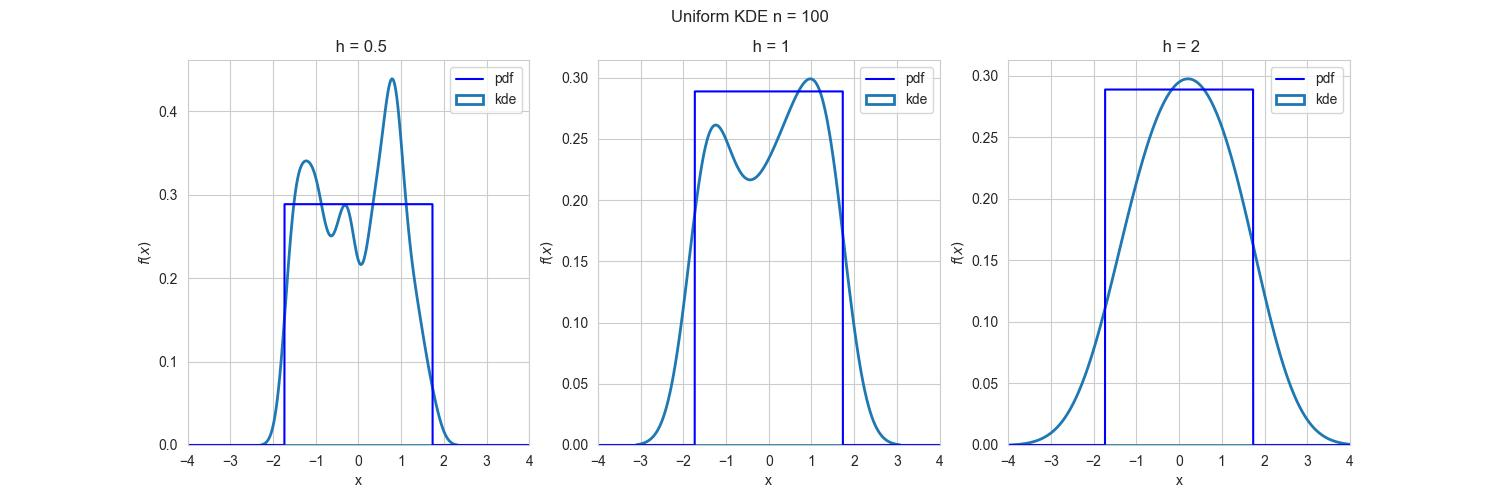
\includegraphics[scale=0.45]{task_4/resource/Uniform KDE100.jpg}}
		\caption{Равномерное распределение, $n=100$} 
		\label{fig:normal}
	\end{figure}